\chapter{Related work}

\section{A fast method for simulating destruction and the generated dust
and debris}
This method \cite{edem} approaches destruction on three scales. At first, the destruction is performed on a coarse scale, and then the applied energy is used to calculate the amount and size of smaller debris and finally dust particles.

\begin{enumerate}
\item Destruction on coarse scale \\ on this level we use Extended Distinct Element Method (EDEM) which is based on Element Method described in the first chapter. The behaviour of the entire system is calculated based on interactions of individual elements. EDEM extends the method formerly using only contact force by adding pore springs connecting the adjacent elements. If we imagine the elements as individual bricks than the pore springs represent a mortar holding them together. If the applied force is sufficient and elements move apart far enough, the fraction takes place. Pore springs also help the object retain its original shape after applied force.
\begin{figure}[ht!]
        \centering
        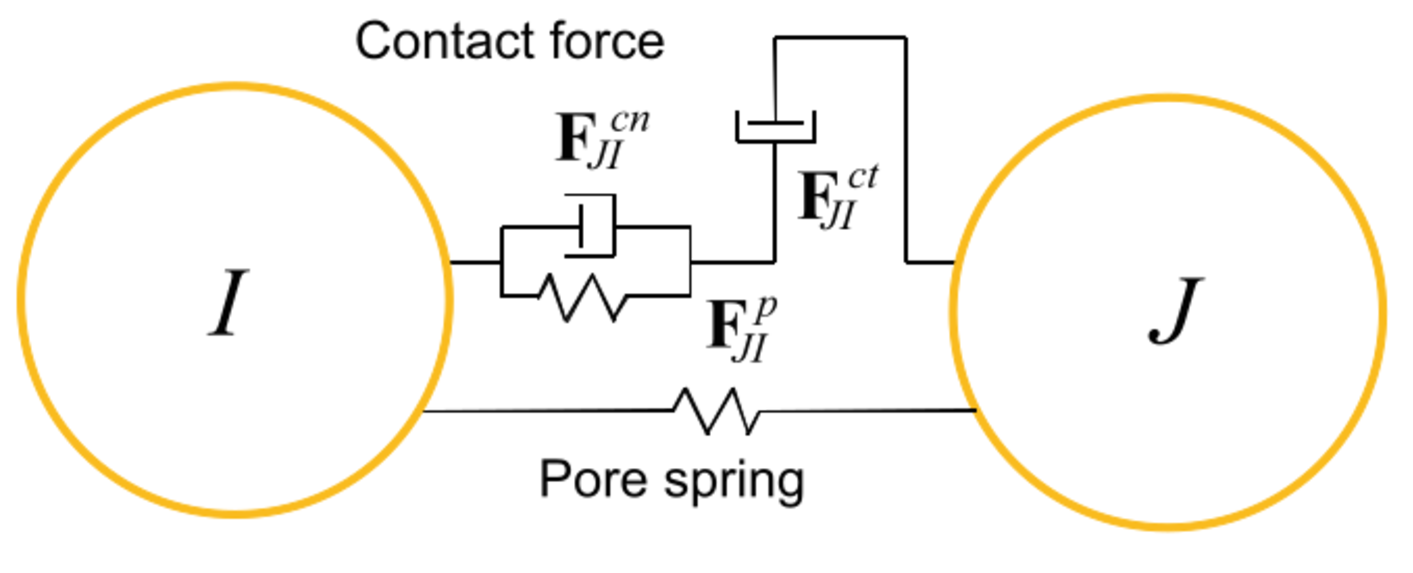
\includegraphics[width=0.7\textwidth]{img/spring}
        \caption{The force between two EDEM elements \cite{edem}}
        \label{spring}
\end{figure}
\\Algorithm for creating EDEM elements
\begin{enumerate}
\item Represent the original object as a closed surface model.
\item Arbitrarily arrange the EDEM elements inside the object.
The elements are allowed to overlap at this point.
\item Move the elements by performing the EDEM simulation. However, we only consider the contact force in this simulation.
\item Perform collision detection between the object’s surface
and the elements, making sure that the elements always
stay inside the object.
\item Repeat (3)–(4) until the elements are stabilised.
\item Construct a Delaunay diagram from the set of elements
and put the pore springs on the Delaunay edges that connect
the elements
\end{enumerate}
The position $\mathbf{x}_I$ and velocity $\mathbf{v}_I$ of the element $\mathit{I}$ can be found using Newton’s equation of motion as follows:
 
\[M\frac{d\mathbf{v}_I}{dt} = \sum_{J \in contact}^{} \mathbf{F}_{JI}^c + \sum_{K \in pore}^{} \mathbf{F}_{KI}^p + M\mathbf{g} \]
\[ \frac{d\mathbf{x}_I}{dt} = \mathbf{v}_I \]
Here, $\mathbf{g}$ is the gravitational vector, $\mathbf{F}^c_{JI}$ is the contact force, $\mathbf{F}^p_{KI}$ is the force due to the pore springs and $\mathit{M}$ is the element’s mass. Contact contains elements \{I, J\} if they are closer than the diameter of a single element, while pore
contains a pair of elements \{I, K\} when they are connected by a pore spring.

\item Fine debris generation and simulation \\after fracture between EDEM elements we can determine if the energy was big enough to break EDEM element into smaller debris. The Gaudin-Schuhmann distribution is used to determine the size of debris. Debris is taken out of EDEM simulation and put into particle simulation, where each piece is represented as a particle without volume.

\item Dust generation and simulation \\ amount of generated dust is based on fracture energy and results of debris generation. Instead of simulating particles smaller than predetermined margin, they are represented as dust in a grid-based fluid simulation. The density of particular cell represents the amount of dust.

\end{enumerate}

 \begin{figure}[ht!]
        \centering
        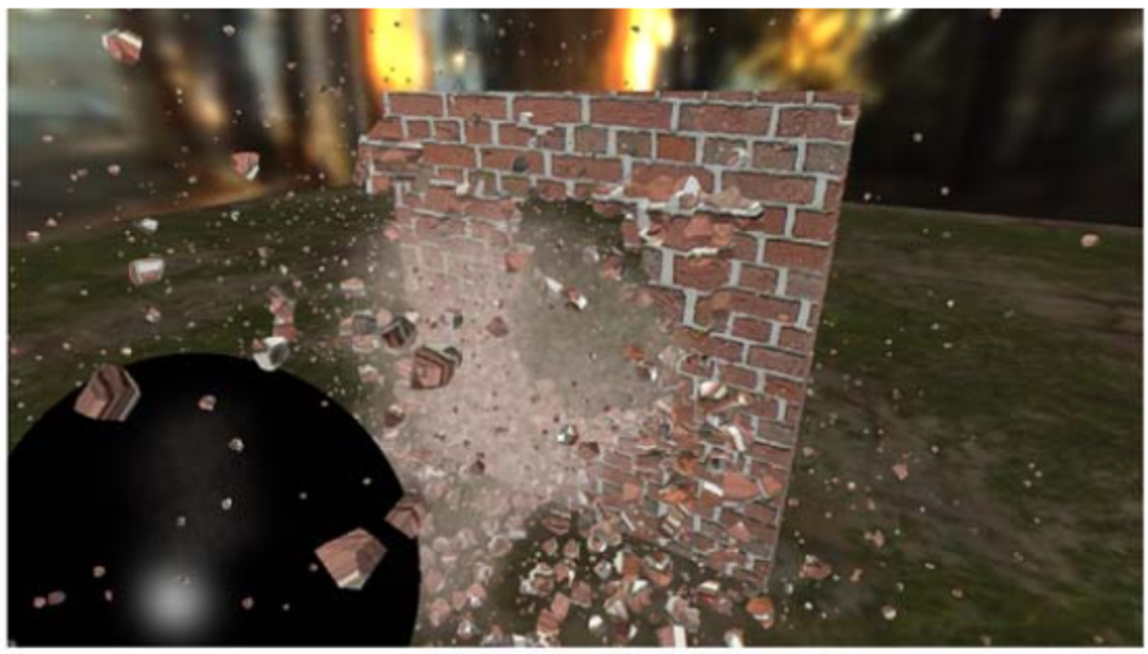
\includegraphics[width=0.49\textwidth]{img/edem_real}
        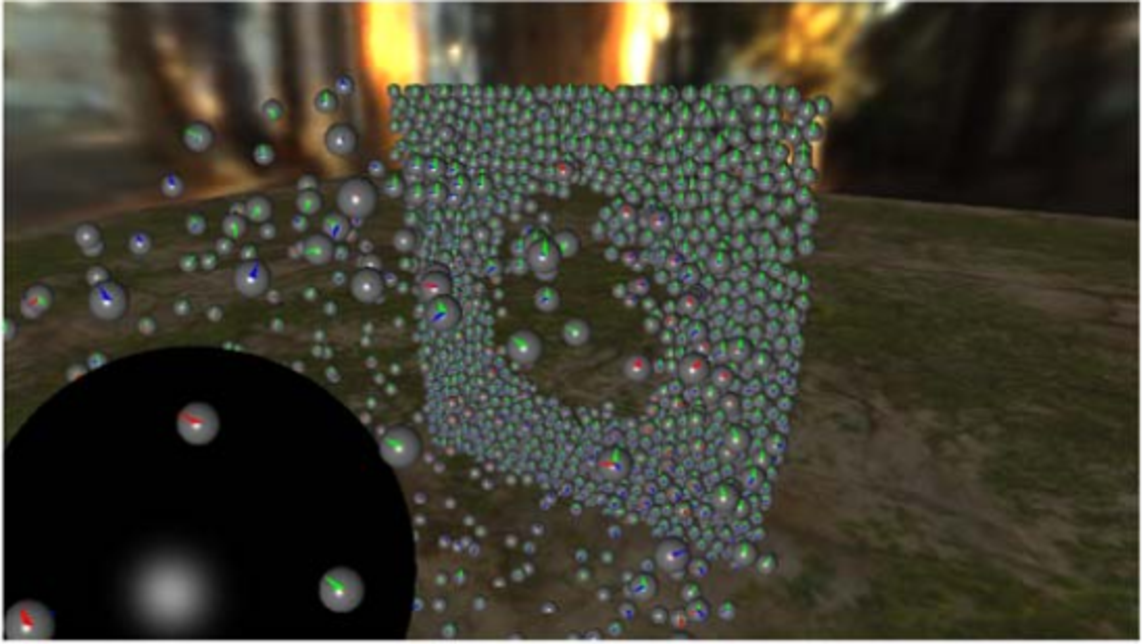
\includegraphics[width=0.49\textwidth]{img/edem}
        \caption{Result of this method with generated dust and debris (left) and EDEM elements (right) \cite{edem}}
        \label{edem}
    \end{figure}
   
\begin{table}[ht!]
    \begin{center}
  \begin{tabular}{ |l|c|c|c|c|c| } 
  \hline
  EDEM elements & 128 & 256 & 512 & 1024 & 2048 \\ 
  \hline
  FPS & 320 & 160 & 75 & 30 & 9.1 \\ 
  \hline
  
  \end{tabular}
  \end{center}
  \caption{Performance of EDEM element method without rendering \cite{edem}}
  \label{table1}
\end{table}
In conclusion, based on table \ref{table1}, the frames per second (fps) drop proportionally with growing number of EDEM elements. That makes this approach unusable in large scale environments in real time game which demands constant 30fps at least.

\section{Real Time Dynamic Fracture
with Volumetric Approximate Convex Decompositions}
\cite{nvidia}


















